\chapter{More on Functions}
%\addcontentsline{toc}{chapter}{1 Graphs}
%%%%%%%%%%%%%%% SECTION HEADER %%%%%%%%%%%%%%%%
\rhead{2}
\lhead{More on Functions}
%%%%%%%%%%%%%%%%%%% START %%%$%%%%%%%%%%%%%%%%%
\section{Increasing and decreasing functions}
If the function \textit{rises from left to right}, the function is called \textbf{increasing}. On the other hand, if the function \textit{falls from left to right}, the function is called \textbf{decreasing}.
\begin{figure}[ht]
    \centering
    \subfloat[Increasing function]{{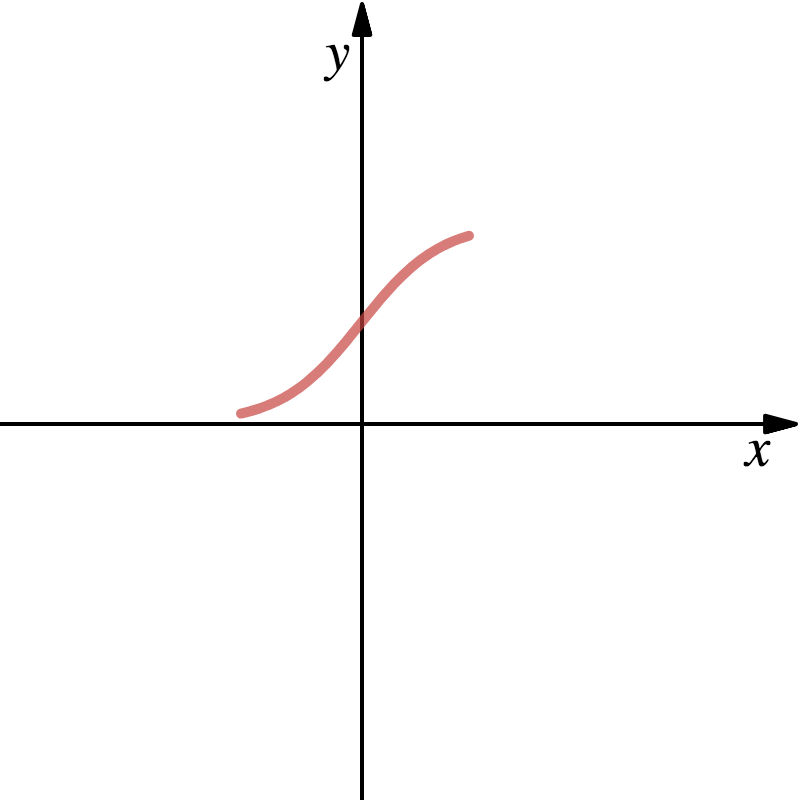
\includegraphics[width=4cm]{Pics/increasing.png} }}%
    \qquad
    \subfloat[Decreasing function]{{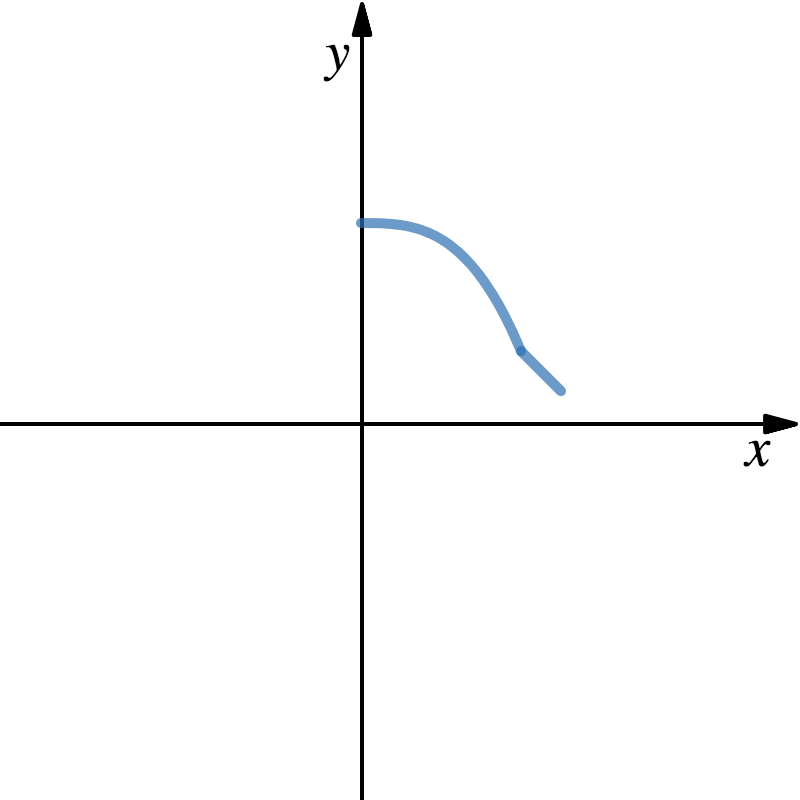
\includegraphics[width=4cm]{Pics/decreasing.png} }}%
    \caption{Increasing and decreasing function}%
    \label{fig:inc_dec}%
\end{figure}


If the function \textit{neither rise nor fall} and remains constant, it is called \textbf{constant}. Constant function is a horizontal line.
\begin{figure}[ht]
    \centering
    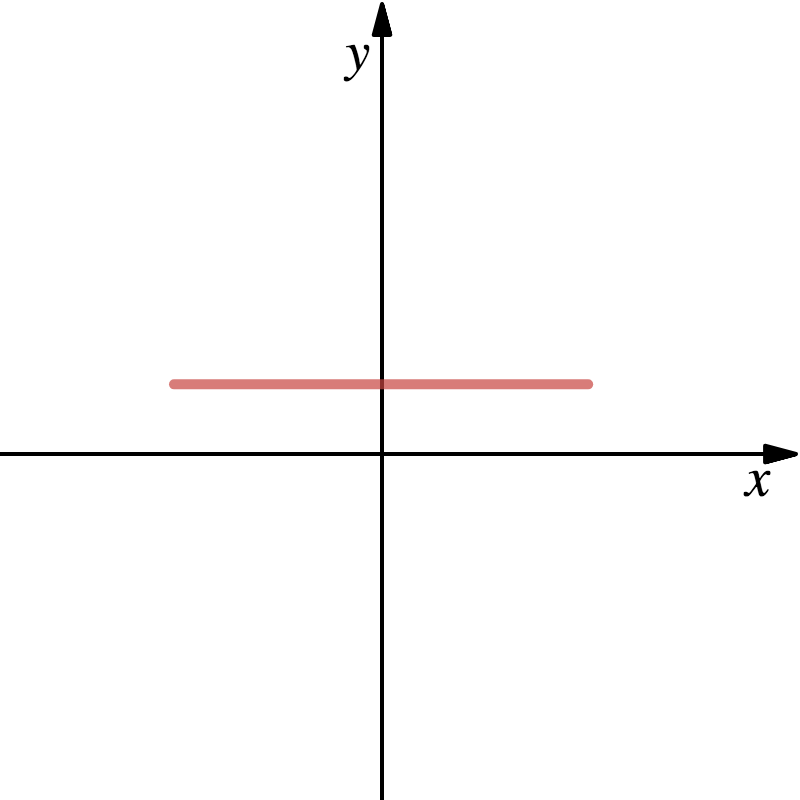
\includegraphics[width=5cm]{Pics/constant.png}
    \caption{Constant function is a horizontal line.}
    \label{fig:const}
\end{figure}
% ====== EXAMPLE 1
\begin{exa}
    State the intervals on which the given function is increasing, decreasing, or constant.
\end{exa}
\begin{center}
\begin{tikzpicture}
\begin{axis}[my style, 
        minor tick num=1,
        xmin=-6,xmax=6,ymin=-26,ymax=26, samples=100]
  \addplot +[<->, mark=none, blue, ultra thick, domain=-3:3] (x,x*x*x-3*x);
\end{axis}
\end{tikzpicture}
\end{center}
As you can see, the function rises from $-\infty$ to $-1$. Then start falling from $-1$ to $1$. Finally, it rises again from $1$ to $+\infty$. So
\begin{align*}
        (-\infty,\, -1)&    &&\text{Increasing}\\
        (-1,\, 1)&  &&\text{Decreasing}\\
         (1,\, +\infty)& &  &\text{Increasing}
\end{align*}
% ========= SECTION
\section{Difference Quotient}
The difference quotient gives us the slope of line between the  two points of $x$ and $x+h$:
\begin{equation}
        \text{Difference quotient}=\frac{f(x+h)-f(x)}{h}\\
        \label{diff_quotient}
\end{equation}
This value is actually the average rate of change of a function. Later in calculus, once you learn limit, you will find out that this expression becomes the slope of a tangent line at any point of the graph when $h$ approaches to $0$. In this case, this expression is called derivative of a function.
% ========= EXAMPLE
\begin{exa}
    If $f(x) =-2x^2+4x-1$, find and simplify each expression.
    \begin{multicols}{2}
        \begin{enumerate}[(a)]
            \item $f(x+h)$
            \item $\frac{f(x+h)-f(x)}{h}$
        \end{enumerate}
    \end{multicols}
\end{exa}
(a) To find $f(x+h)$ replace $x$ with $x+h$:
\begin{align*}
        f(x+h) &= -2(x+h)^2+4(x+h)-1 \\
        &=-2(x^2+h^2+2xh)+4(x+h)-1\\
        &=-2x^2-2h^2-4xh+4x+4h-1 \quad \checkmark
\end{align*}
(b) We already found $f(x+h)$ from previous part. Substitute both $f(x+h)$ and $f(x)$. Then simplify
\begin{align*}
    &\frac{f(x+h)-f(x)}{h} \\
    &\frac{(-2x^2-2h^2-4xh+4x+4h-1) - (-2x^2+4x-1) }{h}\\
    &\frac{\cancel{-2x^2}-2h^2-4xh+\cancel{4x}+4h-\cancel{1} +\cancel{2x^2}-\cancel{4x}+\cancel{1}) }{h}\\
    &\frac{-2h^2-4xh+4h}{h}\\
    &\frac{\cancel{h}(-2h-4x+4)}{\cancel{h}}\\
    &-2h-4x+4\quad \checkmark
\end{align*}
